\documentclass[ngerman]{beamer}
\usepackage{etex}
\usepackage[beamer]{mydefs}
\usepackage{calc}
\usepackage{babel}
\usepackage{fontspec}
\usepackage{textpos}

%%%

\title{Lernen Terminologischen Wissens\\ mit hoher Konfidenz aus fehlerhaften Daten}
\author{Daniel Borchmann}
\date{9.\,September 2014}

%%%

\includeonlyframes{current}
\usetikzlibrary{decorations.pathmorphing,calc,arrows}
\tikzset{>={stealth'[sep]}}

% \let\oldemph\emph
% \renewcommand{\emph}[1]{\alert<.>{\oldemph{#1}}}

%%%

\begin{document}

\begin{frame}[plain]
  \maketitle
\end{frame}

\begin{frame}

  \onslide<1->

  \begin{block}{Ziel}
    Wissen aus Daten für maschinelle Bearbeitung extrahieren
  \end{block}

  \onslide<2->

  \begin{block}{Beobachtung}
    \begin{itemize}
    \item<3-> faktisches Wissen leicht extrahierbar
    \item<8-> terminologisches (begriffliches) Wissen schwer extrahierbar
    \end{itemize}
  \end{block}

  \onslide<4->

  \vspace*{-0.6\baselineskip}
  \begin{overlayarea}{\linewidth}{13ex}
    \only<4-6>{
      \begin{Beispiel}[DBpedia/Wikidata]
        \only<5->{
          \begin{center}\ttfamily
            <http://dbpedia.org/resource/\alert<6->{Aldous\_Huxley}>\\
            <http://dbpedia.org/ontology/\alert<6->{notableWork}>\\
            <http://dbpedia.org/resource/\alert<6->{Brave\_New\_World}> .
          \end{center}
        }
      \end{Beispiel}
    }
    
    \only<9->{
      \begin{Beispiel}
        \begin{itemize}
        \item<10-> Jede Katze ist ein Säugetier
        \item<11-> Hunde sind keine Katzen
        \item<12-> Jeder Mensch, der ein Kind hat, ist ein Elternteil
        \end{itemize}
      \end{Beispiel}
    }
  \end{overlayarea}

\end{frame}

\begin{frame}

  \onslide<1->

  \begin{block}{Grundlegende Fragen}
    \begin{itemize}
    \item<2-> Wie Wissen darstellen? \visible<5->{$\quad\Rightarrow\quad$
        \emph{Beschreibungslogiken} }
    \item<3-> Wie Wissen extrahieren? \visible<10->{$\quad\Rightarrow\quad$ \emph{Formale
          Begriffsanalyse}}
    \item<4-> Welches Wissen extrahieren? \visible<11->{$\quad\Rightarrow\quad$
        \emph{\enquote{interessantes}}}
    \end{itemize}
  \end{block}

  \onslide<6->

  \begin{Beispiel}[General Concept Inclusions, GCIs]
    \begin{itemize}
    \item<7-> $\mathsf{Cat} \sqsubseteq \mathsf{Mammal}$
    \item<8-> $\mathsf{Dog} \sqcap \mathsf{Cat} \sqsubseteq \bot$
    \item<9-> $\exists \mathsf{child}. \top \sqsubseteq \mathsf{Parent}$
    \end{itemize}
  \end{Beispiel}

\end{frame}

\begin{frame}

  \onslide<+->
  
  \centering
  
  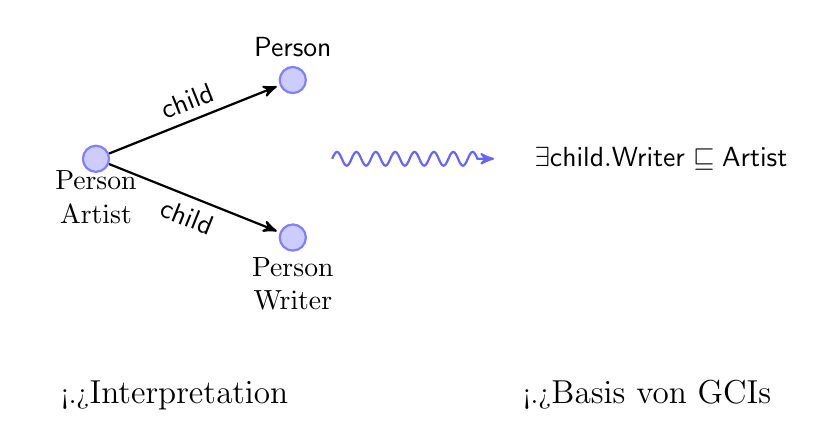
\begin{tikzpicture}[element/.style = {circle,draw=blue!50,fill=blue!20,thick}]
    \node[element, draw, circle, label=below:{\parbox{1.5cm}{\vspace*{-.5cm}\center
        Person\\Artist}}] (B) at (3,-1) {};
    \node[element, draw, circle, label=above:{\sf Person}] (C) at (5.5,0) {};
    \node[element, draw, circle, label=below:{\parbox{1.5cm}{\vspace*{-.4cm}\center
        Person\\Writer}}] (D) at (5.5,-2) {};
    \path[->,thick]
    (B) edge node[midway,above,sloped] {\sf child} (C)
    (B) edge node[midway,below,sloped] {\sf child} (D)
    ;

    \node[coordinate] (D) at (6,-1) {};

    \onslide<+->{
      \node  (E) at (10,-1) {$\quad\mathsf{\exists child.Writer} \sqsubseteq \mathsf{Artist}$};
      \draw[->,thick,blue!60,opaque=50,decorate,decoration={coil,aspect=0,post length=0.7em,
        segment length=0.7em}] (D) to (E);
    }

    \onslide<+->{
      \node at (4, -4) {\alert<.>{\large Interpretation}};
    }

    \onslide<+->{
      \node at (10, -4) {\alert<.>{\large Basis von GCIs}};
    }
  \end{tikzpicture}
  
\end{frame}

\begin{frame}

  \onslide<+->

  Fixiere disjunkte Mengen $N_{C}$ (Konzeptnamen) und $N_{R}$ (Rollennamen).

  \onslide<+->

  \begin{Definition}
    \emph{$\ELbot$-Konzeptbeschreibungen} $C$ sind von der Form
    \begin{equation*}
      C ::= A \mid C \sqcap\! C \mid \exists r. C \mid \bot \mid \top
    \end{equation*}
    für $A \in N_C, r \in N_R$.
  \end{Definition}

  \onslide<+->

  \begin{Beispiel}
    \begin{equation*}
      \mathsf{Cat} \sqcap \mathsf{Dog}, \exists \mathsf{child}. \mathsf{Writer}, \top, \bot
    \end{equation*}
  \end{Beispiel}

\end{frame}

\begin{frame}

  \onslide<+->

  \begin{Definition}
    Eine \emph{Interpretation} $\mathcal{I} = (\Delta^{\mathcal{I}}, \cdot^{\mathcal{I}})$
    besteht aus
    \begin{itemize}
    \item<+-> einer nicht-leeren Menge $\Delta^{\mathcal{I}}$ von \emph{Elementen},
    \item<+-> einer Abbildung $\cdot^{\mathcal{I}}$ mit
      \begin{align*}
        A^{\mathcal{I}} &\subseteq \Delta^{\mathcal{I}} \\
        r^{\mathcal{I}} &\subseteq \Delta^{\mathcal{I}} \times \Delta^{\mathcal{I}}
      \end{align*}
      für $A \in N_{C}, r \in N_{R}$.
    \end{itemize}
  \end{Definition}

  \onslide<+->

  \begin{Definition}
    Für $A \in N_C$, $C, D$ zwei $\ELbot$-Konzeptbeschreibungen und $r \in N_R$ sei
    \begin{itemize}
    \item $\bot^{\mathcal{I}} = \emptyset$, $\top^{\mathcal{I}} = \Delta^{\mathcal{I}}$,
    \item $(C \sqcap D)^{\mathcal{I}} := C^{\mathcal{I}} \cap D^{\mathcal{I}}$,
    \item $(\exists r. C)^{\mathcal{I}} := \set{ x \in \Delta^{\mathcal{I}} \mid \exists y
        \in \Delta^{\mathcal{I}} \st (x, y) \in r^{\mathcal{I}}, y \in C^{\mathcal{I}} }$.
    \end{itemize}
  \end{Definition}

\end{frame}

\begin{frame}

  \onslide<+->

  \begin{Definition}
    Sind $C, D$ zwei $\ELbot$-Konzeptbeschreibungen, so heißt
    \begin{equation*}
      C \sqsubseteq D
    \end{equation*}
    \emph{Allgemeine Konzeptinklusion} (General Concept Inclusion, GCI).

    \onslide<+->%
    \medskip{}
    $C \sqsubseteq D$ \emph{gilt} in $\mathcal{I}$ falls
    \begin{equation*}
      C^{\mathcal{I}} \subseteq D^{\mathcal{I}}.
    \end{equation*}
  \end{Definition}

\end{frame}

\begin{frame}

  \onslide<+->
  
  \begin{Definition}
    $\con K = (G, M, I)$ heißt \emph{formaler Kontext}, falls $G, M$ Mengen und $I
    \subseteq G \times M$.

    \onslide<+->\medskip

    Für $A \subseteq G, B \subseteq M$ sei
    \begin{align*}
      \only<+->{A' &= \set{ m \in M \mid \forall g \in A \holds (g, m) \in I },} \\
      \only<+->{B' &= \set{ g \in G \mid \forall m \in B \holds (g, m) \in I }}
    \end{align*}
  \end{Definition}
  
  \onslide<+->

  \begin{Definition}
    $A \to B$ heißt \emph{Implikation} in $\con K$, falls $A, B \subseteq M$. \onslide<+->
    $A \to B$ heißt \emph{gültig} in $\con K$, falls
    \begin{equation*}
      A' \subseteq B'.
    \end{equation*}
  \end{Definition}
  
\end{frame}

\begin{frame}

  \onslide<+->

  \begin{block}{Offene Frage}
    Was ist \enquote{interessantes} Wissen?
  \end{block}

  \onslide<+->

  \begin{block}{Erste Idee \textcolor{gray}{[Baader, Distel 2009]}}
    \onslide<+->
    Betrachte alle \emph{gültigen} GCIs \onslide<+-> $\Longrightarrow$ berechne
    \emph{Basis} aller gültigen GCIs.
  \end{block}

  \onslide<+->

  \begin{block}{Beobachtung}
    \begin{itemize}
    \item<+-> GCIs sind Implikationen sehr ähnlich
    \item<+-> FCA bietet Möglichkeiten, Implikationen aus Daten zu berechnen
    \end{itemize}
    \onslide<+->%
    $\Longrightarrow$ FCA-Methoden verallgemeinern
  \end{block}

\end{frame}

\newcommand{\datacloud}{
  \begin{scope}[every node/.style={coordinate},scale=.4]
    \node (A) at (0,0) {};
    \node (B) at (2,3) {};
    \node (C) at (4,5) {};
    \node (D) at (6,3) {};
    \node (E) at (7,1) {};
    \node (F) at (5,-1) {};
    \node (G) at (3,-1.5) {};
    \node (H) at (2,-1) {};
    \draw [every edge/.style={bend left}, every to/.style={bend left=70}]
    (A) to (B) to (C) to (D) to (E) to (F) to (G) to (H) to (A);

    \path {
      node  (A1) at ( 4.96,  0.31) {}
      node  (A2) at ( 5.81,  0.82) {}
      node  (A3) at ( 6.82, -0.39) {}
      node  (A4) at ( 3.72, -0.40) {}
      node  (A5) at ( 2.80,  3.60) {}
      node  (A6) at ( 2.43, -0.38) {}
      node  (A7) at ( 3.84,  3.23) {}
      node  (A8) at ( 4.32,  2.23) {}
      node  (A9) at ( 3.79, -0.97) {}
      node (A10) at ( 6.26, -0.01) {}
      node (A11) at ( 4.91,  0.95) {}
      node (A12) at ( 0.17, -3.22) {}
      node (A13) at ( 3.17,  4.53) {}
      node (A14) at ( 4.11,  5.49) {}
      node (A15) at ( 4.44,  5.18) {}
      node (A16) at ( 2.65, -1.27) {}
      node (A17) at ( 6.50,  1.66) {}
      node (A18) at ( 6.50,  1.12) {}
      node (A19) at ( 0.33,  5.20) {}
      node (A20) at ( 3.39,  5.00) {}
      node (A21) at ( 4.25,  5.55) {}
      node (A22) at ( 4.85, -1.15) {}
      node (A23) at ( 4.79,  0.90) {}
      node (A24) at ( 0.32, -2.88) {}
      node (A25) at ( 7.57,  5.03) {}
      node (A26) at ( 5.58,  0.94) {}
      node (A27) at (-0.08,  2.98) {}
      node (A28) at ( 1.65,  4.32) {}
      node (A29) at ( 0.28, -3.43) {}
      node (A30) at ( 2.47,  3.51) {}
      node (A31) at ( 4.58, -3.49) {}
      node (A32) at ( 4.39, -3.34) {}
      node (A33) at ( 7.06,  4.72) {}
      node (A34) at ( 0.25,  4.98) {}
      node (A35) at ( 4.35,  4.47) {}
      node (A36) at ( 3.26,  5.40) {}
      node (A37) at ( 7.85,  2.42) {}
      node (A38) at ( 3.45, -2.30) {}
      node (A39) at (-0.99, -0.57) {}
      node (A40) at ( 6.99,  3.45) {}
      node (A41) at ( 2.98,  6.02) {}
      node (A42) at ( 4.41,  2.02) {}
      node (A43) at ( 3.54, -2.62) {}
      node (A44) at ( 3.10, -2.21) {}
      node (A45) at ( 6.03,  1.45) {}
      node (A46) at ( 1.96,  6.39) {}
      node (A47) at ( 0.80,  2.64) {}
      node (A48) at ( 3.93,  2.99) {}
      node (A49) at ( 5.50,  3.82) {}
      node (A50) at ( 2.55,  0.24) {}
      node (A51) at ( 5.19,  0.94) {}
      node (A52) at ( 5.38, -3.34) {}
      node (A53) at ( 2.70,  4.65) {}
      node (A54) at ( 4.79, -3.16) {}
      node (A55) at ( 3.94,  0.30) {}
      node (A56) at ( 0.43, -0.20) {}
      node (A57) at ( 0.08,  2.96) {}
      node (A58) at ( 5.88, -2.67) {}
      node (A59) at (-0.31,  3.40) {}
      node (A60) at ( 5.53, -2.33) {}
      node (A61) at ( 0.65,  3.93) {}
      node (A62) at ( 1.02,  6.56) {}
      node (A63) at ( 1.67,  1.63) {}
      node (A64) at ( 5.52, -1.86) {}
      node (A65) at ( 0.71,  2.94) {}
      node (A66) at ( 1.15,  0.47) {}
      node (A67) at ( 5.53,  2.78) {}
      node (A68) at ( 1.74, -1.02) {}
      node (A69) at ( 5.33, -3.23) {}
      node (A70) at ( 1.05,  2.35) {}
      node (A71) at ( 0.50,  2.10) {}
      node (A72) at ( 1.00,  0.15) {}
      node (A73) at ( 1.31,  6.55) {}
      node (A74) at ( 2.63,  5.41) {}
      node (A75) at ( 3.90,  6.48) {}
      node (A76) at (-0.41, -0.38) {}
      node (A77) at ( 3.87,  0.63) {}
      node (A78) at ( 2.56, -0.55) {}
      node (A79) at ( 3.29, -0.31) {}
      node (A80) at ( 6.97,  4.80) {}
      node (A81) at ( 3.72,  5.67) {}
      node (A82) at (-0.59,  3.14) {}
      node (A83) at ( 5.67,  5.28) {}
      node (A84) at ( 5.80,  2.08) {}
      node (A85) at ( 5.20,  5.49) {}
      node (A86) at ( 2.25, -0.03) {}
      node (A87) at ( 1.49, -0.80) {}
      node (A88) at ( 1.40,  0.01) {}
      node (A89) at ( 1.14,  0.76) {}
      node (A90) at ( 3.22,  2.07) {}
      node (A91) at (-1.79,  2.54) {}
      node (A92) at ( 7.97,  3.17) {}
      node (A93) at ( 4.48,  3.51) {}
      node (A94) at ( 5.64,  1.88) {}
      node (A95) at ( 5.25,  3.42) {}
      node (A96) at ( 4.12,  6.62) {}
      node (A97) at ( 4.74,  5.57) {}
      node (A98) at ( 2.47,  3.29) {}
      node (A99) at ( 7.62,  4.09) {}
    };

    \draw[->,lightgray] {
      (A93) -- (A52)
      (A16) -- (A97)
      (A76) -- (A69)
      (A91) -- (A46)
      (A97) -- (A13)
      (A16) -- (A8)
      (A91) -- (A85)
      (A37) -- (A92)
      (A72) -- (A52)
      (A27) -- (A21)
      (A56) -- (A50)
      (A10) -- (A14)
      (A65) -- (A72)
      (A14) -- (A26)
      (A65) -- (A63)
      (A42) -- (A43)
      (A74) -- (A12)
      (A13) -- (A27)
      (A21) -- (A63)
      (A26) -- (A80)
      (A46) -- (A86)
      (A58) -- (A98)
      (A61) -- (A6)
      (A96) -- (A59)
      (A6)  -- (A49)
      (A4)  -- (A74)
      (A23) -- (A41)
      (A36) -- (A6)
      (A32) -- (A13)
      (A31) -- (A86)
      (A86) -- (A59)
      (A77) -- (A3)
      (A82) -- (A54)
      (A58) -- (A93)
      (A91) -- (A31)
      (A1)  -- (A43)
      (A26) -- (A87)
      (A47) -- (A3)
      (A6)  -- (A14)
      (A7)  -- (A51)
      (A35) -- (A34)
      (A81) -- (A68)
      (A48) -- (A21)
      (A52) -- (A59)
      (A59) -- (A18)
      (A22) -- (A8)
      (A53) -- (A98)
      (A94) -- (A72)
      (A43) -- (A34)
      (A40) -- (A7)
      (A1)  -- (A78)
      (A31) -- (A9)
      (A6)  -- (A71)
      (A36) -- (A40)
      (A22) -- (A32)
      (A57) -- (A78)
      (A50) -- (A65)
      (A6)  -- (A81)
      (A73) -- (A75)
      (A78) -- (A34)
      (A70) -- (A82)
      (A54) -- (A17)
      (A40) -- (A5)
      (A99) -- (A26)
      (A55) -- (A76)
      (A3)  -- (A38)
      (A32) -- (A6)
      (A17) -- (A90)
      (A29) -- (A30)
      (A78) -- (A80)
      (A68) -- (A12)
      (A63) -- (A95)
      (A14) -- (A46)
      (A65) -- (A31)
      (A64) -- (A14)
      (A10) -- (A62)
      (A3)  -- (A92)
      (A55) -- (A57)
      (A66) -- (A37)
      (A81) -- (A87)
      (A74) -- (A75)
      (A28) -- (A56)
      (A6)  -- (A12)
      (A64) -- (A16)
      (A53) -- (A4)
      (A48) -- (A21)
      (A23) -- (A52)
      (A13) -- (A87)
      (A44) -- (A33)
      (A51) -- (A14)
      (A73) -- (A58)
      (A95) -- (A35)
      (A87) -- (A12)
      (A85) -- (A3)
      (A87) -- (A95)
      (A91) -- (A8)
      (A30) -- (A8)
      (A23) -- (A23)
      (A6)  -- (A83)
      (A92) -- (A58)
      (A47) -- (A7)
      (A59) -- (A41)
      (A88) -- (A33)
      (A6)  -- (A60)
      (A7)  -- (A15)
      (A95) -- (A45)
      (A58) -- (A40)
      (A35) -- (A42)
      (A81) -- (A90)
      (A57) -- (A48)
      (A48) -- (A23)
      (A23) -- (A74)
      (A7)  -- (A46)
      (A14) -- (A37)
      (A11) -- (A81)
      (A95) -- (A31)
      (A9)  -- (A73)
      (A58) -- (A16)
      (A95) -- (A47)
      (A29) -- (A36)
      (A17) -- (A36)
      (A29) -- (A89)
      (A5)  -- (A20)
      (A39) -- (A97)
      (A92) -- (A20)
      (A71) -- (A89)
      (A2)  -- (A60)
      (A96) -- (A16)
      (A13) -- (A38)
      (A52) -- (A20)
      (A91) -- (A44)
      (A68) -- (A31)
      (A65) -- (A4)
      (A1)  -- (A13)
      (A49) -- (A10)
      (A4)  -- (A21)
      (A72) -- (A49)
      (A57) -- (A68)
      (A60) -- (A91)
      (A76) -- (A80)
      (A21) -- (A24)
      (A74) -- (A6)
      (A32) -- (A97)
      (A66) -- (A55)
      (A79) -- (A1)
      (A88) -- (A82)
      (A31) -- (A97)
      (A10) -- (A48)
    };

    \foreach \i in {1,...,99} {
      \draw[every node/.style={minimum size=2pt,inner sep=0pt,draw,circle}]
      node at (A\i) {\tiny \i};
    };
    
  \end{scope}
}

\begin{frame}[label=current]

  \onslide<+->
  
  \begin{tikzpicture}
    \datacloud
  \end{tikzpicture}
  
\end{frame}

\begin{frame}

  \onslide<+->
  
  \begin{block}{Experiment}
    \begin{itemize}
    \item<+-> DBpedia: aus der Wikipedia halbautomatisch gewonnenes Wissen
    \item<+-> betrachte nur \textsf{child}-Relation ${} \leadsto \Idbpedia$
    \item<+-> $\Delta^{\Idbpedia} = 5626$
    \end{itemize}
  \end{block}

  \onslide<+->

  \begin{block}{Einige Ergebnisse}
    \vspace*{-3ex}
    \begin{gather*}
      \onslide<+->{\sf MemberOfParliament \sqsubseteq Person \sqcap Politician}~\\
      \onslide<+->{\sf \exists child. Person \sqsubseteq Person}~\\
      \onslide<+->{\sf FictionalCharacter \sqcap \exists child. Person \sqsubseteq \exists
        child. FicitionalCharacter}
    \end{gather*}
  \end{block}

  \onslide<+->

  \vspace*{-3ex}
  \begin{block}{Fragwürdige Ergebnisse}
    \vspace*{-3ex}
    \begin{gather*}
      \onslide<+->{\sf Person \sqcap \exists child. Book \sqsubseteq
        FicitionalCharacter}~\\
      \onslide<+->{\sf Criminal \sqcap \exists child. Politician \sqsubseteq \bot}~\\
      \onslide<+->{\sf Person \sqcap \exists child. Criminal \sqsubseteq Criminal}
    \end{gather*}
  \end{block}

\end{frame}

\begin{frame}
  
  \onslide<1-8>

  \begin{block}{Beobachtung}
    \begin{equation*}
      \sf \exists child. \top \sqsubseteq Person
    \end{equation*}
    \onslide<2->%
    \emph{gilt nicht} in $\Idbpedia$\onslide<3->, denn es gibt 4 \alt<7->{\alert{falsche
        Gegenbeispiele:}}{Gegenbeispiele, \dh}
    \begin{overlayarea}{\textwidth}{5ex}
      \only<4-6>{
        \begin{equation*}
          \abs{ (\sf \exists child.top)^{\Idbpedia} \setminus Person^{\Idbpedia} } = 4.
        \end{equation*}
      }
      \only<8->{
        \begin{equation*}
          \text{\texttt{Teresa\_Carpio}, \texttt{Charles\_Heung},
            \texttt{Adam\_Cheng}, \texttt{Lydia\_Shum}.}
        \end{equation*}
      }
    \end{overlayarea}

    \onslide<5->

    \bigskip{}

    Andererseits: 2547 Elemente in $\Idbpedia$ erfüllen $\sf \exists child. \top
    \sqsubseteq \sf Person$, \dh
    \begin{equation*}
      \abs{ (\sf \exists child.\top \sqcap Person)^{\Idbpedia} } = 2547.
    \end{equation*}

    \onslide<6->

    $\sf \exists child. \top \sqsubseteq Person$ ist also
    \alt<7->{\alert{\enquote{\sout{fast}}}}{\enquote{\makebox[\widthof{\sout{fast}}]{fast}}} richtig.
  \end{block}

\end{frame}

\begin{frame}

  \onslide<+->

  \begin{block}{Intuition}
    Betrachte auch GCIs, die \enquote{fast} richtig sind.
  \end{block}

  \onslide<+->
  \begin{Definition}
    Die \emph{Konfidenz} von $C \sqsubseteq D$ in $\mathcal{I}$ ist gegeben durch
    \begin{equation*}
      \conf_{\mathcal{I}}(C \sqsubseteq D) :=
      \begin{cases}
        1 & \text{falls } C^{\mathcal{I}} = \emptyset,\\
        \frac{\abs{(C \sqcap D)^{\mathcal{I}}}}{\abs{C^{\mathcal{I}}}} & \text{sonst}.
      \end{cases}
    \end{equation*}
    \onslide<+->%
    Sei $c \in [0, 1]$.  Dann
    \begin{equation*}
      \Th_c(\mathcal{I}) := \set{ C \sqsubseteq D \mid \conf_{\mathcal{I}}(C \sqsubseteq
        D) \ge c}.
    \end{equation*}
  \end{Definition}

  \onslide<+->

  \begin{block}{Ansatz}
    Betrachte $\Th_{c}(\mathcal{I})$ als \enquote{interessantes} Wissen in $\mathcal{I}$.
  \end{block}

\end{frame}

\begin{frame}[label=current]

  \onslide<+->
  
  Neue Übersicht, mit Konfidenz
\end{frame}

\begin{frame}

  \onslide<+->

  \begin{block}{Parallels between FCA and DL}
    \begin{center}
      \begin{tabular}{c|c}
        Formal Concept Analysis & Description Logics\\
        \midrule\onslide<+->
        objects $G$ & individuals $\Delta^{\mathcal{I}}$ \\\onslide<+->
        attributes $M$ & concept descriptions \\\onslide<+->
        formal contexts $\con K$ & interpretations $\mathcal{I}$ \\\onslide<+->
        implications & GCIs \\\onslide<+->
        $A', A \subseteq M$ & $(\bigsqcap A)^{\mathcal{I}}$ \\\onslide<+->
        $B', B \subseteq G$ & \textcolor{red}{\textbf{?}}
      \end{tabular}
    \end{center}
  \end{block}

  Details 1: Model-Based Most-Specific Concept Description

  (ELgfp erwähnen)
\end{frame}

\begin{frame}
  Details 2: Kontextkonstruktion, Baader-Distel Resultat
\end{frame}

\begin{frame}
  Details 3: Idee von Luxenburger, Eigenes Resultat
\end{frame}

\begin{frame}
  DBpedia: was kommt dazu?
\end{frame}

\begin{frame}
  Diagramme
\end{frame}

\begin{frame}

  \onslide<+->

  \begin{block}{Problem}
    Ansatz kann \emph{fehlerhafte Daten} von \emph{seltenen Gegenbeispielen} nicht
    unterscheiden.
  \end{block}

  \onslide<+->

  \begin{Beispiel}
    Die Aussage \emph{Alle Säugetieren gebären lebend},
    \begin{equation*}
      \mathsf{Mammal} \sqsubseteq \mathsf{GivesBirth},
    \end{equation*}
    \onslide<+->
    hat Gegenbeispiel \emph{Schnabeltier}
  
    \begin{textblock*}{\linewidth}[0.5,0.5](0.85\linewidth,-1cm)
      \centering
      \includegraphics[width=3cm]{platypus}\\[-2ex]
      {\fontsize{3pt}{4pt}\selectfont http://www.sealifeconservation.org.au/adopt-an-animal/}
    \end{textblock*}

  \end{Beispiel}

  \onslide<+->

  \begin{block}{Ausweg}
    Verwende externe \enquote{Experten}
  \end{block}

\end{frame}

\begin{frame}
  Exploration Übersicht
\end{frame}

\begin{frame}
  Ende und Schluss
\end{frame}

\end{document}

%%% Local Variables: 
%%% mode: latex
%%% TeX-master: t
%%% ispell-local-dictionary: "de_DE"
%%% TeX-engine: xetex
%%% End: 

%  LocalWords:  Wikidata Concept Inclusions Konzeptnamen Rollennamen Konzeptinklusionen
%  LocalWords:  Ableitungsoperatoren Konzeptinklusion Inclusion label current node at
%  LocalWords:  style
